\chapterquote{Empty your mind of any theories,\\ 'Til all the facts are in.}{Death Note Musical}

We define the primary four triangle centers, their corresponding lines, and define a cevian.

\begin{defi}[Cevian]
In a triangle, a cevian is a line segment with a vertex of the triangle as an endpoint and its other endpoint on the opposite side.

\begin{center}
\begin{asy}
size(4cm);
dot((-1,0));
dot((-2,0));
dot((2,0));
dot((1,2));

draw((-2,0)--(2,0)--(1,2)--cycle);
draw((1,2)--(-1,0));

\end{asy}
\end{center}
\end{defi}

\section{Incenter}

The corresponding cevian is the \textit{interior} angle bisector.

\begin{defi}[Interior Angle Bisector]
The interior angle bisector of $\angle CAB$ is the line that bisects acute $\angle CAB.$
\end{defi}

The interior angle bisector of $\angle CAB$ is also the locus of points inside $\angle CAB$ equidistant from lines $AB$ and $AC.$

\begin{fact}[Angle Bisector Equidistant from Both Sides]
In $\angle CAB,$ $\angle PAB=\angle PAC$ if and only if $\delta(P,AB)=\delta(P,AC).$
\end{fact}

\begin{pro}
Let the feet of the altitudes from $P$ to $AB,AC$ be $X,Y.$ Then note that either of these conditions imply $\triangle APX\cong \triangle APY,$ which in turn implies the other condition.
\end{pro}

\begin{theo}[Incenter]
There is a point $I$ that the angle bisectors of $\triangle ABC$ concur at. Furthermore, $I$ is equidistant from sides $AB,BC,CA.$
\end{theo}

\begin{pro}
Recall that a point is on the angle bisector of $\angle CAB$ if and only if $\delta(P,AB)=\delta(P,AC).$ Let the angle bisectors of $\angle CAB$ and $\angle ABC$ intersect at $I.$ Then $\delta(P,CA)=\delta(P,AB)$ and $\delta(P,AB)=\delta(P,BC),$ so $\delta(P,BC)=\delta(P,CA),$ implying that $I$ lies on the angle bisector of $\angle BCA.$

Since $\delta(P,AB)=\delta(P,BC)=\delta(P,CA),$ the circle with radius $\delta(P,AB)$ centered at $I$ is inscribed in $\triangle ABC.$
\begin{center}
    \begin{asy}
import olympiad;
    size(4cm);
    pair A=dir(110);
    pair B=dir(210);
    pair C=dir(-30),D,E,F,I;
    I=incenter(A,B,C);
    D=foot(I,B,C);
    E=foot(I,C,A);
    F=foot(I,A,B);
    dot(A^^B^^C^^I^^D^^E^^F);
    draw(incircle(A,B,C),blue);
    draw(A--B--C--cycle);
    draw(A--I--B);
    draw(I--C,red);
    draw(I--D,dotted);
    draw(I--E,dotted);
    draw(I--F,dotted);
    label("A",A,dir(90));
    label("B",B,dir(200));
    label("C",C,dir(-20));
    label("D",D,dir(-90));
    label("E",E,dir(35));
    label("F",F,dir(135));
    label("I",I,dir(60));
    \end{asy}
\end{center}
\end{pro}

\section{Centroid}

The corresponding cevian is the median.

\begin{defi}[Midpoint]
The midpoint of segment $AB$ is the unique point $M$ that satisfies the following:
\begin{enumerate}[label=(\alph*)]
    \item $M$ is on $AB.$
    
    \item $AM=MB.$
\end{enumerate}
\end{defi}

\begin{defi}[Median]
The $A$-median of $\triangle ABC$ is the line segment that joins $A$ with the midpoint of $BC.$
\end{defi}

\begin{theo}[Centroid]
The medians $AD,BE,CF$ of $\triangle ABC$ concur at a point $G.$ Furthermore, the following two properties hold:
\begin{enumerate}[label=(\alph*)]
    \item $\frac{AG}{GD}=\frac{BG}{GE}=\frac{CG}{GF}=2.$
    
    \item $[BGD]=[CGD]=[CGE]=[AGE]=[AGF]=[BGF].$
\end{enumerate}

\end{theo}

\begin{pro}
Let $BE$ intersect $CF$ at $G.$ Since $\triangle AFE\sim \triangle ABC,$ $FE\parallel BC.$ Thus $\triangle BCG\sim\triangle EFG$ with a ratio of $\frac{BC}{EF}=2,$ so $\frac{BG}{GE}=2.$

Similarly let $BE$ intersect $AD$ at $G'.$ Repeating the above yields $\frac{BG'}{G'E}=2.$ Thus $G$ and $G'$ are the same point, and the medians are concurrent.

\begin{center}
    \begin{asy}
    import olympiad;
    size(5cm);
    pair A=dir(110), B=dir(200), C=dir(-20), D,E,F,G;
    G=(A+B+C)/3;
    D=(B+C)/2;
    E=(C+A)/2;
    F=(A+B)/2;
    dot(A^^B^^C^^D^^E^^F^^G);
    draw(A--B--C--A);
    draw(E--F);
    draw(B--E);
    draw(C--F);
    label("A",A,N);
    label("B",B,dir(190));
    label("C",C,dir(-10));
    label("D",D,S);
    label("E",E,dir(45));
    label("F",F,dir(140));
    label("G",G,dir(90));
    \end{asy}
\end{center}
\end{pro}

\section{Circumcenter}

A perpendicular bisector is not a cevian, but it is still a special line in triangles.

\begin{defi}[Perpendicular Bisector]
The perpendicular bisector of a line segment $AB$ is the locus of points $X$ such that $AX=BX.$
\end{defi}

The circumcenter is the unique circle that contains points $A,B,C.$

\begin{theo}[Circumcenter]
There is a point $O$ that the perpendicular bisectors of $BC,CA,AB$ concur at. Furthermore, $O$ is the center of $(ABC).$
\end{theo}

\begin{pro}
Let the perpendicular bisectors of $AB,BC$ intersect at $O.$ By the definition of a perpendicular bisector, $AO=BO$ and $BO=CO.$ But this implies $CO=AO,$ so $O$ lies on the perpendicular bisector of $CA.$

Since $AO=BO=CO,$ the circle centered at $O$ with radius $AO$ circumscribes $\triangle ABC.$

\begin{center}
    \begin{asy}
    import olympiad;
    size(4cm);
    pair A=dir(110);
    pair B=dir(210);
    pair C=dir(-30),D,E,F,I;
    I=circumcenter(A,B,C);
    D=foot(I,B,C);
    E=foot(I,C,A);
    F=foot(I,A,B);
    dot(A^^B^^C^^I^^D^^E^^F);
    draw(circumcircle(A,B,C),blue);
    draw(A--B--C--cycle);
    draw(A--I--B,dotted);
    draw(I--C,dotted);
    draw(I--D);
    draw(I--E,red);
    draw(I--F);
    label("A",A,dir(90));
    label("B",B,dir(200));
    label("C",C,dir(-20));
    label("D",D,dir(-90));
    label("E",E,dir(35));
    label("F",F,dir(135));
    label("O",I,dir(95));
    \end{asy}
\end{center}
\end{pro}

\section{Orthocenter}

The corresponding cevian is the altitude.

\begin{defi}[Altitude]
The $A$-altitude of $\triangle ABC$ is the line through $A$ perpendicular to $BC.$
\end{defi}

\begin{defi}[Foot of Altitude]
The foot of the altitude from $A$ to $BC$ is the point $H$ where the $A$-altitude intersects $BC.$
\end{defi}

\begin{theo}[Orthocenter]
The altitudes of $\triangle ABC$ concur.
\end{theo}

\begin{pro}
We will be piggybacking on the proof for the circumcenter.

Let the line through $B$ parallel to $AC$ and the line through $C$ parallel to $AB$ intersect at $D.$ Define $E,F$ similarly. Note that $FA=BC=AE,$ so the $A$ altitude of $\triangle ABC$ is the perpendicular bisector of $DE.$ Since the circumcenter exists, the orthocenter must too.

\begin{center}
    \begin{asy}
    import olympiad;
    size(4cm);
    pair A=dir(110), B=dir(200), C=dir(-20), D,E,F,H;
    H=orthocenter(A,B,C);
    D=B+C-A;
    E=C+A-B;
    F=A+B-C;
    dot(A^^B^^C^^D^^E^^F^^H);
    draw(A--B--C--A);
    draw(D--E--F--D);
    draw(A--H,dotted);
    draw(B--H,dotted);
    draw(C--H,dotted);
    label("A",A,N);
    label("B",B,dir(190));
    label("C",C,dir(-10));
    label("D",D,S);
    label("E",E,dir(45));
    label("F",F,dir(140));
    label("H",H,dir(35));
    \end{asy}
\end{center}
\end{pro}

\section{Summary}

\subsection{Theory}

\begin{enumerate}
\item Angle Bisector
\begin{itemize}
\Item The angle bisector bisects the angle, as the name suggests.

\Item It is also the locus of points equidistant from two lines.
\end{itemize}

\item Incenter
\begin{itemize}
\Item The incenter is the center of the incircle.

\Item The incenter is equidistant from all sides.

\Item The incenter is the concurrence point of the angle bisectors.
\end{itemize}

\item Median
\begin{itemize}
\Item The median joins the vertex to the midpoint of the opposite side.
\end{itemize}

\item Centroid
\begin{itemize}
\Item The centroid is the center of mass.

\Item The centroid is the concurrence point of the medians.

\Item The centroid $G$ splits the medians in the ratio $\frac{AG}{GD}=2$.
\end{itemize}

\item Perpendicular Bisector
\begin{itemize}
\Item The perpendicular bisector is the locus of points equidistant from the endpoints of a line segment.

\Item The perpendicular bisector perpendicularly bisects the segment.
\end{itemize}

\item Circumcenter
\begin{itemize}
\Item The circumcenter is the center of the circumcircle.

\Item The circumcenter is equidistant from all vertices.

\Item The circumcenter is the concurrence point of the perpendicular bisectors.
\end{itemize}

\item Altitude
\begin{itemize}
\Item The altitude is the perpendicular line through one vertex to the opposite side.

\Item The foot of the altitude is the intersection of the altitude with the side.
\end{itemize}

\item Orthocenter
\begin{itemize}
\Item The orthocenter is the concurrence point of the altitudes.
\end{itemize}
\end{enumerate}

\subsection{Tips and Strategies}

\begin{enumerate}
\item Incenter
\begin{itemize}
\Item Just remember that the angle bisector bisects angles.
\end{itemize}

\item Centroid
\begin{itemize}
\Item Length chase with the length condition.

\Item Take homotheties from the midpoint of a side with scale factor $\frac{1}{3}$ to send the opposite vertex to the centroid.

\Item Remember that the medians split the triangle into six triangles of equal area.
\end{itemize}

\item Circumcenter
\begin{itemize}
\Item Use $AO=BO=CO$ to find isosceles triangles - this will help a lot with angle chasing.
\end{itemize}

\item Orthocenter
\begin{itemize}
\Item Watch out for right triangles and right angles.
\end{itemize}
\end{enumerate}

\pagebreak

\section{Exercises}

\subsection{Check-ins}

\begin{enumerate}
    \item Prove that a triangle is equilateral if and only if its incenter is the same point as its circumcenter.
    
    \item Consider $\triangle ABC$ with incenter $I.$ Prove that $\angle BIC=90^{\circ}+\frac{1}{2}\angle BAC.$
    \begin{hint}
    \begin{addhint}
    {Look at $\triangle BIC.$}
    \end{addhint}
    \end{hint}
    
    \item Prove that the perpendicular bisector of line segment $AB$ is perpendicular to and bisects $AB,$ if the perpendicular bisector is defined as the locus of points $X$ such that $AX=BX.$
    
    \item Consider $\triangle ABC$ with circumcenter $O.$ If $AO=20$ and $BC=32,$ find $[BOC].$
    
    \item (AMC 10A 2020/12) Triangle $AMC$ is isosceles with $AM = AC$. Medians $\overline{MV}$ and $\overline{CU}$ are perpendicular to each other, and $MV=CU=12$. What is the area of $\triangle AMC?$
    
    \begin{center}
        \begin{asy}
import olympiad;
size(4cm);
draw((-4,0)--(4,0)--(0,12)--cycle);
draw((-2,6)--(4,0));
draw((2,6)--(-4,0));
label("M", (-4,0), W);
label("C", (4,0), E);
label("A", (0, 12), N);
label("V", (2, 6), NE);
label("U", (-2, 6), NW);
label("P", (0, 3.6), S);
\end{asy}
    \end{center}
\end{enumerate}

\subsection{Problems}

\begin{enumerate}
	\item (AMC 10B 2018/12) Line segment $\overline{AB}$ is a diameter of a circle with $AB=24$. Point $C$, not equal to $A$ or $B$, lies on the circle. As point $C$ moves around the circle, the centroid (center of mass) of $\triangle{ABC}$ traces out a closed curve missing two points. To the nearest positive integer, what is the area of the region bounded by this curve?
\begin{solu}
\begin{addsol}
{Let $O$ be the center of the circle and $G$ be the centroid of $\triangle ABC.$ Since $O$ is also the midpoint of $AB$ and thus lies on $CG$, we're motivated to make use of the $2:1$ ratio. $CO$ always has length $12,$ so it follows that $GO$ always has length $4.$ This means that the locus of $G$ is a circle with center $O$ and radius $4$ by definition, so the area is $16\pi\approx 50.$

\begin{center}
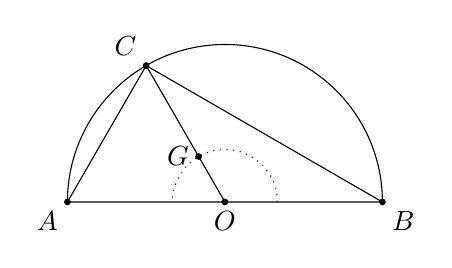
\begin{tikzpicture}
\draw (0,0)--(4,0)--(1,1.73205081)--cycle;
\draw (1,1.73205081)--(2,0);
\filldraw (0,0) circle (1pt) node[anchor= north east] {$A$};
\filldraw (4,0) circle (1pt) node[anchor=north west] {$B$};
\filldraw (1,1.73205081) circle (1pt) node[anchor=south east] {$C$};
\filldraw (2,0) circle (1pt) node[anchor= north] {$O$};
\filldraw (1.66666,0.57735027) circle (1pt) node[anchor= east] {$G$};
\draw (4,0) arc (0:180:2);
\draw[dotted] (8/3,0) arc (0:180:2/3);
\end{tikzpicture}
\end{center}}
\end{addsol}
\end{solu}

	\item Let $\triangle ABC$ have medians $BM,CN,$ and let $P$ and $Q$ be the feet of the altitudes from $B,C$ to $CN,BM,$ respectively. Prove that the quadrilateral $MNPQ$ is cyclic.
	\begin{hint}
	\begin{addhint}
	{Use Power of a Point.}
	\end{addhint}
	\begin{addhint}
	{Show that $GP\cdot GN=GQ\cdot GM,$ where $G$ is the centroid of $\triangle ABC.$}
	\end{addhint}
	\begin{addhint}
	{Remember that the centroid splits the median in a fixed ratio.}
	\end{addhint}
	\end{hint}
	\begin{solu}
	\begin{addsol}
	{Let the centroid be $G.$ We want to prove that $XP\cdot XN=XQ\cdot XM,$ which is equivalent to proving $XP\cdot XC=XQ\cdot XB,$ as $\frac{XC}{XN}=\frac{XB}{XM}=2.$ Now note that $BPQC$ is cyclic as $\angle BPC=\angle BQC=90^{\circ},$ which finishes the problem.}
	\end{addsol}
	\end{solu}

    \item Consider $\triangle ABC$ with medians $BE,CF.$ If $BE$ and $CF$ are perpendicular, find $\frac{b^2+c^2}{a^2}.$\begin{hint}
    \begin{addhint}
    {Look at $\triangle GBC.$}
    \end{addhint}
    \begin{addhint}
    {You can get $BE$ and $BF$ (via Stewart's), so you can get $BG$ and $CG.$}
    \end{addhint}
    \end{hint}
    \begin{solu}
    \begin{addsol}
    {By Stewart's, $BE=\frac{\sqrt{2c^2+2a^2-b^2}}{2}$ and $CF=\frac{\sqrt{2a^2+2b^2-c^2}}{2},$ so $a^2=BG^2+CF^2=\frac{4}{9}(\frac{2c^2+2a^2-b^2}{4}+\frac{2a^2+2b^2-c^2}{4})=\frac{4a^2+b^2+c^2}{9}.$
    
    Thus, $5a^2=b^2+c^2$ and $\frac{b^2+c^2}{a^2}=5.$}
    \end{addsol}
    \end{solu}
    
    \item (Brazil 2007) Let $ABC$ be a triangle with circumcenter $O$. Let $P$ be the intersection of straight lines $BO$ and $AC$ and $\omega$ be the circumcircle of triangle $AOP$. Suppose that $BO = AP$ and that the measure of the arc $OP$ in $\omega$, that does not contain $A$, is $40^{\circ}$. Determine the measure of the angle $\angle OBC$.
    \begin{hint}
    \begin{addhint}
    {Note that $BO=AO.$}
    \end{addhint}
    \begin{addhint}
    {$\triangle AOP$ is isosceles.}
    \end{addhint}
    \end{hint}
    \begin{solu}
    \begin{addsol}
    {Note that $BO=AO=AP,$ so $\triangle AOP$ is isosceles. Thus $\angle OAP=20^{\circ},$ implying $\angle AOC=140^{\circ},$ and $\angle AOP=\angle APO=80^{\circ},$ implying that $\angle AOB=100^{\circ}.$ So $\angle OBC=360^{\circ}-140^{\circ}-100^{\circ}=120^{\circ},$ or $\angle OBC=30^{\circ}.$
    
    \begin{center}
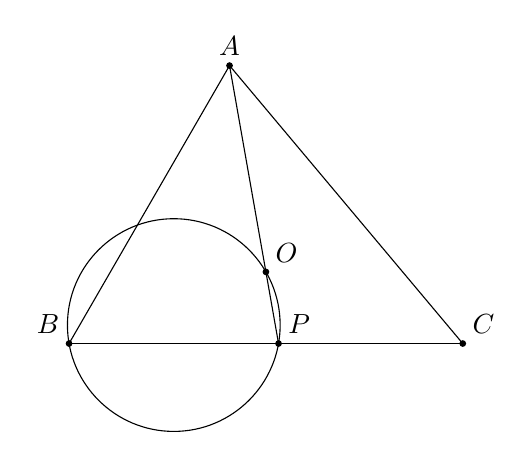
\begin{tikzpicture}
\draw (0.,0.)-- (5.,0.);
\draw (2.038018672739762,3.529951887959356)-- (0.,0.);
\draw (2.660444431189779,0.)-- (2.038018672739762,3.529951887959356);
\draw (2.038018672739762,3.529951887959356)-- (5.,0.);
\draw (1.3302222155948895,0.23455406694717237) circle (1.3507430374366678cm);

\filldraw (0.,0.) circle (1pt) node[anchor=south east] {$B$};
\filldraw (5.,0.) circle (1pt) node[anchor=south west] {$C$};
\filldraw (2.038018672739762,3.529951887959356) circle (1pt) node[anchor=south] {$A$};
\filldraw (2.5,0.9099255856655059) circle (1pt) node[anchor=south west] {$O$};
\filldraw (2.660444431189779,0.) circle (1pt) node[anchor=south west] {$P$};
\end{tikzpicture}
    \end{center}}
    \end{addsol}
    \end{solu}
\end{enumerate}

\subsection{Challenges}

\begin{enumerate}
    \item Three congruent circles $\omega_1,\omega_2,\omega_3$ concur at $P.$ Let $\omega_1$ intersect $\omega_2$ at $A\neq P,$ let $\omega_2$ intersect $\omega_3$ at $B\neq P,$ and let $\omega_3$ intersect $\omega_1$ at $C\neq P.$ What triangle center is $P$ with respect to $\triangle ABC?$
    
    \item Let $ABC$ be an isosceles triangle with $AB=AC.$ If $\omega$ is inscribed in $ABC$ and the orthocenter of $ABC$ lies on $\omega,$ find $\frac{AB}{BC}.$

    \item Let $G$ be the centroid of $\triangle ABC.$ If $\angle BGC=90^{\circ},$ find the maximum value $\sin A$ can take.
    \begin{hint}
    \begin{addhint}
    {Have you found $\frac{b^2+c^2}{a^2}$ yet?}
    \end{addhint}
    \end{hint}
\end{enumerate}